%!TEX root = ../thesis.tex

\chapter{Introduction}
\label{chap:i}

\section{Motivation}
\label{sec:motivation}

[Section to be written.]

[Text below copied from P2; to be adapted.]

Constructing and maintaining an up-to-date graph-like road network on the national level has a range of firmly established uses. Owing to its structure, it can be used efficiently for modelling and simulation purposes, such as for traffic flow simulations, passenger transport modelling, construction and upgrade impact modelling (to pinpoint optimal locations and types of investment), and traffic noise load modelling (\cite{bell_lida_1997, zhu_li_2007, zhang_2011, duran_santos_2014, peng_etal_2020}). It can also be used for navigation; a graph-like road network representation is at the heart of most road navigation services (\cite{yue_etal_2008}). Combined with other data sets, we can mention an even wider range of use cases: complemented by ecological statistics and models, it can offer insight into the impact of the presence of roads, and planned road construction on the flora and fauna in their vicinity. Or to mention logistical benefits, a good model representing the road network in a digital format may be used as a shared working space when aggregating geospatial data relating to road infrastructure from various sources. It makes it possible for geographical road locations, topographical relationships, and arbitrary semantic information to reside in the same network-type data model, making analysis techniques more straightforward, enforcing consistency and saving effort for data providers who would otherwise all need to maintain their own road model (\cite{ekpenyong_etal_2007}).

One may remark that a two-dimensional representation with approximate geographical locations may suffice for many of these purposes, topology being the main concern in network analysis. For instance, GNSS navigation software often use snapping methods to ensure that the navigating vehicle always traverses the road graph – ensuring that even for imperfect road locations and positioning, the navigation remains continuous (\cite{fouque_bonnifait_2008, chen_hsu_2020}). Traffic flow simulations are primarily concerned with traffic loads, road properties, and how roads are subdivided by intersections, among many other aspects. \textit{Mostly}, they are not concerned with the exact geographical locations of roads – as long as the lengths of the roads are correct, any geographical permutation will yield invariant results (\cite{thomson_richardson_1995}).

However, some applications are concerned with the road network in the context of its surroundings, which makes the accuracy of its georeferencing a relevant topic. Noise modelling is one such example, because the propagation of road noise is sensitive to the height of the road itself as well as to the immediate surroundings of the roads, requiring exact geographical locations of non-road objects surrounding the road (such as buildings or noise barriers), and terrain (\cite{ishiyama_etal_1991, bennett_1997, guarnaccia_quartieri_2012}). However, a 2D representation of the road network can only describe lateral positions, a factor that may limit its use in applications where elevation is important. For instance, consider two buildings at the side of a road, a tall one \textit{behind} a shorter one. A 2D semantic road model would tell us that the entirety of the taller building receives a decreased noise load, because the shorter one – positioned between the taller building and the road – suppresses it. In reality, this observation is invalid because the part of the taller building which is visible from the road above the shorter building receives the full noise load. To be able to represent such 3D relationships in our model correctly, we need both buildings and roads to be truly three-dimensional.

2D-projected digital road models with mediocre accuracy have attracted great scientific and commercial attention since the advent of digital cartography and satellite navigation (\cite{taylor_etal_2001, fouque_bonnifait_2008, yue_etal_2008, chen_hsu_2020}). However, \textit{accurate 3D representations} are still atypical, owing to factors such as increased cost of generation and maintenance, increased complexity of visualisation and analysis, and a lack of significant use cases (\cite{zhu_li_2007, wang_etal_2014}). As a result, 2D road models are common in terms of both public and private geospatial providers, whereas accurate 3D road models are rare in comparison.

When a use case arises and an accurate 3D model is needed, the provider generally faces two choices: to produce a new model, or to enrich an existing 2D model with elevation data. The decision generally depends on the quality of the available 2D data set relative to the requirements for the 3D model, as well as that of the dataset(s) available as sources of elevation data, with which the 2D model can be enriched, among other factors (\cite{zhu_li_2007, zhu_li_2008, wang_etal_2014}). In terms of the source of elevation data, the rule of thumb in the geospatial field is that data acquisition is far more expensive than re-using existing datasets, especially openly available ones. As a result, many providers first attempt to find a way to convert their datasets into 3D using existing data in such a cost-effective manner.

\section{The NDW commission}
\label{sec:commission}

[Section to be written.]

[Text below copied from P2; to be adapted.]

In certain projects the accuracy requirement and restrictions on the modelling procedure may be prescribed legally. Such is the case for the client of the proposed MSc dissertation research, the \textit{Nationaal Dataportaal Wegverkeer} (NDW, National Road Traffic Data Portal), part of \textit{Rijkswaterstaat} (RWS, Directorate-General for Public Works and Water Management), a Dutch government organisation who are in the process of enriching their pre-existing open data 2D road model, called \textit{Nationaal Wegenbestand} (NWB, National Road Database), with 3D data, to attain compliance with \textit{SWUNG2}, the new version of the Dutch noise legislation or \textit{geluidwetgeving}. The new version of this legislation prescribes, among other things, accuracy requirements for the road model underlying the noise simulations, with explicit mention of it having to be three-dimensional. Due to cost considerations and reasons related to NDW’s data acquisition pipeline, the pre-existing 2D realisation of NWB will be converted into a 3D dataset (dubbed \textit{3D-NWB}) primarily using open data geospatial datasets. They have produced a prototype realisation themselves, and subsequently contracted the consultant firm \textit{Royal HaskoningDHV} (RHDHV) to create a commercial implementation based on their experience with the prototype. The development of this tool was concluded in December 2020. In addition to simply using the commercial implementation, they wish to assess how it fares in terms of spatial accuracy-related SWUNG2-compliance. This dissertation research will attempt to contribute to this assessment by producing an original implementation that favours accuracy, and in which accuracy can be \textit{tracked} and \textit{quantitatively evaluated}. This implementation will also serve as a reference to which its commercial counterpart can be compared so that its accuracy can be evaluated indirectly, and will also explore various related geomatics topics in the process. This document presents the preliminary findings and project plans of the proposed research.

\section{Commercial project}
\label{sec:commercial}

[Section to be written.]

\section{Preparation}
\label{sec:prep}

[Section to be written.]

\section{Field and relevance}

I will primarily focus on a Lidar point cloud and a 3D topographical line dataset as elevation sources. In both of these datasets, it is evidenced that roads are in truly three-dimensional relationships with one another and with their environment. For instance, they cross above and below other roads and are often constructed underground, in tunnels. The question arises, how such real-world geometries should be dealt with in the conversion process. The answer to this question defines which field of geoscience my project is positioned in. The two candidates in the context of digital road network modelling are GIS and geomatics. It is thus worth discussing briefly how each typically treats 3D objects. One of the reasons why 2D road models are popular is that their geometry and network properties can be analysed using a multitude of well-proven GIS methods and software kits. However, in GIS models, even if elevation measurements exist, they are generally only present as an \textit{elevation attribute} (i.e. a semantic data field, like street names), because GIS geometrical models do not typically support true 3D operations. This is conceptually identical to projecting the geometries onto the horizontal plane. Geometric models that treat the vertical dimension explicitly are more common in geomatics; namely 2.5D and 3D models. While using 2.5D models restricts the types of physical entities that can be modelled, it also greatly simplifies certain types of analysis conceptually and computationally. This makes it ideal for modelling on similar scales to GIS; on the national scale for instance, as in this research. While 2.5D modelling initially appears to be a good candidate for this project, we may observe that it is by definition unsuitable for handling the 3D relationships that roads have with each other and with their environment. However, much like how the concept of divide-and-conquer works in computer science, it is possible decompose 3D problems into smaller sub-problems until they become natively compatible with 2.5D methods. This research is positioned in the geomatics field because my implementation will explore how 2.5D methods can be applied in a way that enables the \textit{piecewise} modelling of a national road network. The divide-and-conqer concept will be applied to decompose the road network into segments that can be individually, locally regarded as \textit{terrain} and hence be modelled in 2.5D. As the proposed research focuses on 2.5D methods to a great extent, it overlaps with the geomatics field of digital terrain modelling in terms of how it will generate and store the digital representation of road surfaces, and as a consequence, the manner in which it will derive elevations from them. As the Methodology section (\ref{sec:m}) will reveal, it also strongly overlaps with the geomatics field of 3D feature extraction (and to a small extent, photogrammetry), because of how I propose to derive the 2.5D road surface models from our input datasets. As also indicated in the Research questions section (\ref{sec:rq}), it is among the specific aims of this project to study how a combination of mainly geomatics-based tools and methods can be used to accomplish the tasks required by NDW, as well as to assess their accuracy and suitability when used in this way.

\section{Research questions}
\label{sec:rq}

[Section below copied from P2; to be revised.]

My main research question is \textit{"How can we achieve a 3D conversion of the NWB dataset using Dutch open geospatial data and a primarily 2.5D-based surface modelling methodology, while guaranteeing optimal and quantifiable accuracy and completeness?"}. As I already mentioned in Section \ref{sec:rw}, combining this question with an awareness of which exact datasets I will be able to use suggests two sub-topics: identifying a combination of primarily 2.5D geomatics methods that could be used to complete the 3D enrichment of NDW, and ensuring and quantifying output accuracy. The research questions I present below are separated into two groups accordingly.

\begin{enumerate}
    \item How is it possible to \textit{perform and benchmark} the elevation-enrichment of NWB using Dutch open geospatial data and an efficient, predominantly 2.5D-based geomatics set of methods?
    \begin{enumerate}
        \item What are the exact methods of the commercial implementation? What do we suspect the theoretical shortcomings to be, based on RHDHV's methods and output?
        \item What types of research have been carried out in this particular field? What can we learn from existing research? How successful were the related research projects?
        \item Can my methods be built around the same datasets as the ones used in the commercial implementation? What are the characteristics of these datasets?
        \item Is it possible to base the workflow entirely on 2.5D methods by decomposing this intrinsically 3D problem into a collection of smaller problems? Can such a method of decomposition also be used to solve the scaling issues related to handling a national Lidar point cloud input dataset?
        \item How well does the implementation perform in areas of complex 3D road relationships? How can this performance be assessed visually and quantitatively using real-world examples, such as multi-level motorway exchanges and roads on long, elevated civil engineering structures?
        \item Is it possible to build the workflow in a way that it allows efficient update operations to be carried out as new data arrives or old data is updated?
        \item How do temporal inconsistencies manifest themselves in the procedure, and in the output? What problems may arise, and how best to solve them?
        \item How well does the implementation perform in areas where input elevation data is scarce, or missing? How can this performance best be assessed visually and quantitatively using real-world examples, such as dense vegetation cover or other objects occluding roads, and roads constructed in tunnels?
        \item How can we best assess the overall performance of the implementation against the commercial implementation in locations that are expected to be difficult to work with, such as where data is scarce?
        \item How smooth is the output? Are sudden jumps introduced after aggregating the decomposed model? If so, can this be resolved by optimising the procedure, or are additional smoothing steps necessary?
        \item Can the same workflow be used to also derive elevations for lines that lie a fixed distance away from the NWB centrelines, representing the \textit{vicinity} of roads?
        \item Can the workflow be used to optimise the \textit{horizontal} location of NWB centrelines?
        \item Can the workflow serve as an aggregator of elevation data originating from small scale sources such as road management datasets?
        \item The workflow is planned to produce surface models of \textit{road segments}. What would be needed to aggregate these into a global model containing all roads?
    \end{enumerate}
    \item Can the processing workflow be developed in a way that it can guarantee optimal \textit{completeness and accuracy}, based on a scientifically sound quantification thereof?
    \begin{enumerate}
        \item What types of accuracy may we distinguish between? Topological accuracy? Lateral accuracy? Purely elevation accuracy? How does each type of uncertainty affect the output? Is uncertainty also influenced by geographically variable factors?
        \item In pre-existing research, what methods have been used to measure accuracy and estimate the influence of processing steps on accuracy?
        \item What is the accuracy of our elevation sources? Can we trust elevation data sources with undocumented accuracy?
        \item What is the effect of uncertainty in the lateral positions of NWB centrelines? Could the impact of this be reduced by optimising the lateral location of NWB?
        \item What do we need to be able to track the evolution of the accuracy throughout the workflow? Can we build it exclusively from steps that prevent serious degradation to the accuracy, while making any degradation quantifiable?
        \item How does the addition of small-scale elevation data sources influence accuracy? How can they be best made use of in this context?
        \item Would it be possible to develop the solution in a way that it can automatically indicate where levels of uncertainty drop below the prescribed threshold, and why?
        \item If smoothing steps are necessary as a post-processing step, how can we be certain that the vertical displacements do not corrupt accuracy? Are topological constraints necessary? If so, how can they be enforced?
        \item How may we measure or estimate the accuracy of the commercial implementation? Can it be tracked throughout their procedure starting from input accuracy, or is it necessary to rely on more indirect methods?
    \end{enumerate}
\end{enumerate}

\section{Research plan}
\label{sec:rq}

[Section to be written.]

[I could re-use the Gantt-chart from the P2 here.]

The following page contains a diagram illustrating the schedule of my graduation year. Please note that the exact P3, P4 and P5 dates are not yet known, hence the week in which they are shown in the diagram are tentative. As a result, the overall length of time available in the second semester is also not yet fixed; the longest possible time is shown.

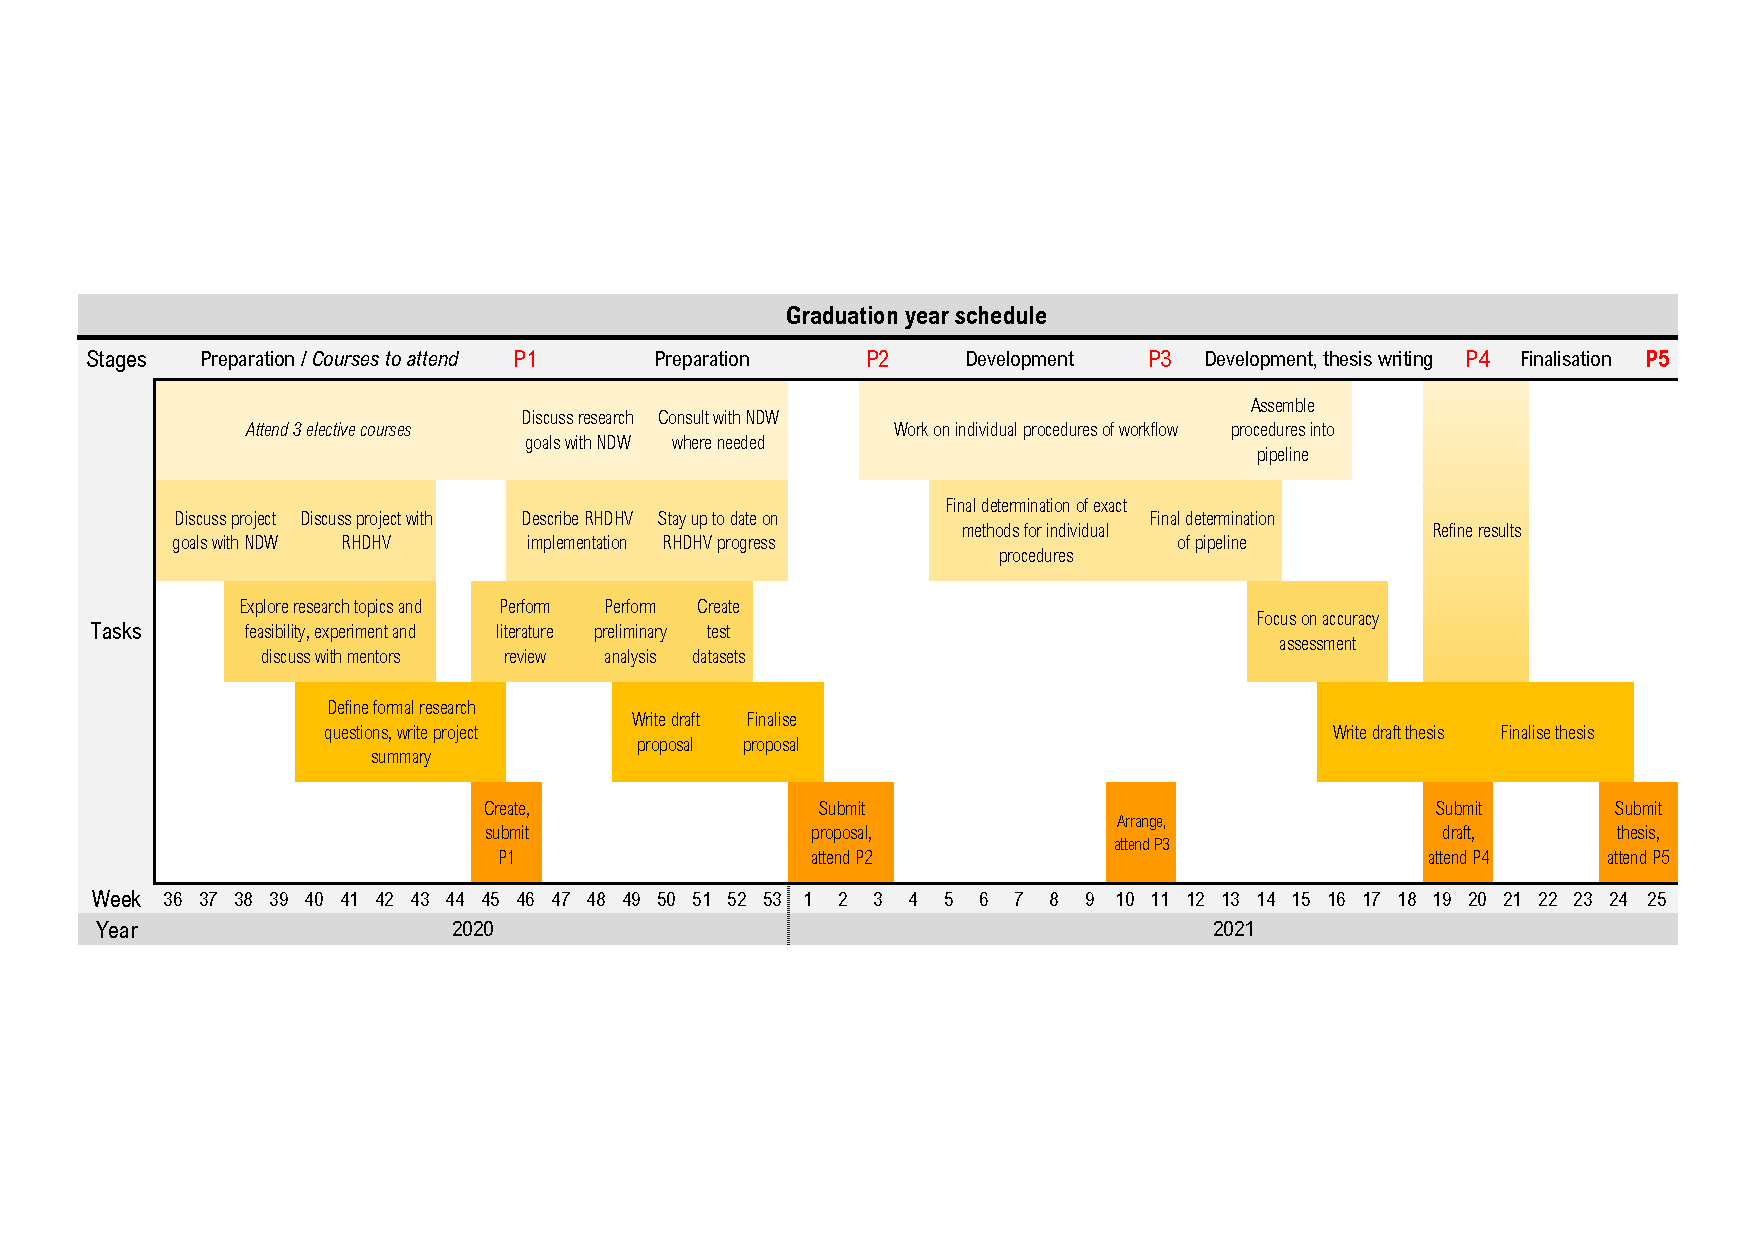
\includepdf[landscape=true]{figs/project_schedule_a4.pdf}